\documentclass[12pt,letterpaper]{article}

%%%%%%%%%%%%%%%%%%%%%%%%%%%%%%%%%%%%%%%%%%%%%%%%%%%%%%%%%%%%%%%%%%%%%%%%%%%%%%%%%%%%%%%%%%%%%%%%%%%%%
% This is the preamble.  It's the place where you load extra packages to enable 
% more functionality.

\usepackage{epigraph}                %for nicely formatting epigraphs
\usepackage{graphicx}                %for inputing images
\usepackage{siunitx}                 %for nicely formatting numbers
\usepackage{threeparttable}          %workaround to get footnotes in tables
\usepackage{adjustbox}               %to make the tables fit
\usepackage{caption}                 %to allow customizing captions to not have numbers with caption*
\usepackage{fancyhdr}                %to control where I want the page numbers
\setlength{\headheight}{14.5pt}      %to make sure the header height is sufficient
\usepackage{pdfpages}                %for easy full page images
\usepackage{pgfplots}                %to plot bar charts
\pgfplotsset{compat=1.6}          %you should request which version of pgfplot you want
\usepackage{pgf-pie}                 %to easily make pie charts
\usepackage[margin=1.25in]{geometry} %for easily controlling margin size
\usepackage[parfill]{parskip}        %for increasing default space between paragraphs
\usepackage[hidelinks,pdftex,colorlinks]{hyperref}     %for all the links
\usepackage{xcolor}
% \hypersetup{colorlinks=false}      %uncomment if you don't want hyperlinks coloured
\setlength{\parindent}{0pt}          %no space at start of paragraphs

%%%%%%%%%%%%%%%%%%%%%%%%%%%%%%%%%%%%%%%%%%%%%%%%%%%%%%%%%%%%%%%%%%%%%%%%%%%%%%%%%%%%%%%%%%%%%%%%%%
% End of preamble.  Next, you start the document with the \begin{document} command.  You have to 
% end the document by closing the document environment: \end{document}.

\begin{document}

\includepdf{odin_wp_cover.pdf} %I only have a crappy version of this from a screenshot

%The title page
\title{\Huge ODIN Blockchain}
\author{Whitepaper v0.1}
\maketitle
\fancyfoot{}
\thispagestyle{fancy}
\renewcommand{\headrulewidth}{0pt}
\newpage

%Contributions page.  
%It's always tricky to get weird formatting right in latex so I fiddle around a little. To get the preface right, I had to define a new command.  There's certainly a better way to do this.  
\newcommand{\MyPrefaceTitle}{%
\begin{center}
\Large 
\textbf{Contributions from}
\normalsize 
\vspace{1cm}
\\
Peter McClory, Darran Trute, Danny Jansen, Vaughn Bullock, Tycho Luyben, Daniel Avital, Rotem Pisam, Kyle Wood, Andre Castagnola, Cameron Brownlee, Joe Carr, Dan Smith, Lucas Howell, Dalton Faguy and many others.
\end{center}
}
\mbox{}
\MyPrefaceTitle  

%Table of contents, with links to pages in document.  I didn't want obvious links in the table of 
%contents, so I coloured them black.
\newpage 
\hypersetup{                         
    linkcolor={black},
    citecolor={blue!50!black},
    urlcolor={blue!80!black}
}                                   
\tableofcontents

%Start of the main document.  Here I thought that hyperlinks would be nicer to have a colour. 
%I also set up the headers and footers for the rest of the document.
\hypersetup{
    linkcolor={blue!80!black},
    citecolor={blue!50!black},
    urlcolor={blue!80!black}
}
\pagestyle{fancy}
\lhead{}
\rhead{}
\cfoot{}
\renewcommand{\headrulewidth}{0pt}
\rfoot[R]{\thepage}


\newpage
\section{Preface}
Cryptographic currencies and decentralized blockchain environments are increasingly pervading industries and society, but still not massively adopted nor in general use. In addition, crypto projects have not typically focused on the mobile environment and privacy is considered a `nice to have' feature.

ODIN aims to address all these concerns. It will do this by:
\begin{itemize}
   \item building a mobile-focused development platform 
   \item creating decentralized applications (Dapps) built on this platform
   \item having privacy as a core feature.
\end{itemize}

The core of ODIN is its community. ODIN will focus on four main communities: the infrastructure community, the Dapps community, the end user community and the entrepreneurial community; all of which require their own information and have different motivations and needs.
\begin{itemize}
\item A committed infrastructure community will provide the backbone of masternodes and staking wallets to ensure resilience, agility and function
\item The Dapps community will provide development in the form of applications to be run by the `end user' community
\item The end user community is our target audience. They download and use the applications built and running on the ODIN Blockchain
\item The entrepreneurial community are interested in ODIN's potential for creating a solution to a known problem and developing this into either a profitable business model or a not-for-profit solution for the common good. Much like the infrastructure community, this community could likely hold a large stake in the network.
\end{itemize}

Developing a Dapp community will help meet ever changing end user needs by creating decentralized applications to enable growth into areas of society where blockchain solutions are needed but not yet provided. One way this Dapp community will be supported is with a range of instructional toolkits and additional support functions. Usability will be at the forefront of every decision, toolkit and tutorial we provide (see \hyperlink{solution}{The Solution}).

A large, diverse and vibrant end user community is the life blood of a utility oriented environment. Adoption patterns guide developers and the service fees resulting from their activity contribute towards the sustainability of the ecosystem as a whole.

The consequential impact of the previous three communities (infrastructure, end user and developer) will ensure continued investment and interest from the entrepreneurial community, and their continued interest in turn yields constant new interest and development within other communities.


\newpage
\section{​The Problem}
\epigraph{\itshape
``At every door-way,\\
ere one enters, \\
one should spy ‘round,\\
one should pry ‘round,\\
for uncertain is the witting\\
that there be no foeman sitting,\\
within, before one on the floor.''}{intro, H\'av\'amal}

ODIN understood the importance of Wisdom. The V\"olusp\`a describes him in the act of  sacrificing one of his eyes in exchange for a single drink from Mimir's well of Wisdom, and thus becoming wiser himself as well.

\subsection{Privacy}
In today's digital age, we find parallels to this. ODIN Blockchain intends to shield the proponents of liberty of thought and ideas from the vision of these aforementioned ``foemen'' and their prying eyes. As Odin sacrificed part of his vision in exchange for knowledge, we plan on obscuring from vision your private conversations and exchanges of thoughts and knowledge. 

Governmental and private institutions are becoming increasingly more adept at gathering data on citizens. It has, in fact, become both a \href{https://patents.google.com/patent/US20110087529A1/en}{science} and a \href{https://patents.google.com/patent/US5974396A/en}{business}. What data to gather and analyze it for practical use. \href{https://www.theguardian.com/news/series/cambridge-analytica-files}{The contemporary media} is full of articles on how \href{https://wikileaks.org/}{lines are being crossed} and how grey areas lack definition.  In addition, passed legislature is allowing for such wide digital surveillance on citizens without justifiable cause, that the old adage ``innocent until proven guilty'' no longer even applies. These laws appear to assume malicious intent from each and every citizen, allowing surveillance on a level that presupposes that we are already suspects in ongoing investigations.

By removing the threat of persecution or worse from the equation, we are encouraging people around the world to contribute to our collective development without fear of censorship.

We believe that, in order to enable a healthy exchange of ideas and thoughts, freedom from persecution and sanctions must be guaranteed when people exercises their simple right to speak. 

Unfortunately, not all institutions around the globe; governmental, private or otherwise, agree with this. Some wish to suppress the exchange of ideas, as it could pose a threat to the powerful. We consider this to be unhealthy for human development as a whole; not just politically, but technologically, spiritually and philosophically as well.

Globally, there is an \href{https://foreignpolicy.com/2010/05/07/the-worlds-top-dissidents/}{abundance of dissidents} that are not allowed to speak under threat of severe consequences to their lives and possibly more.

The ODIN Blockchain will operate in line with Article 17 of the \href{https://www.ohchr.org/EN/ProfessionalInterest/Pages/CCPR.aspx}{International Covenant on Civil and Political Rights} of the United Nations of 1966, stating that: ``No one shall be subjected to arbitrary or unlawful interference with his privacy, family, home or correspondence, nor to unlawful attacks on his honour and reputation. Everyone has the right to the protection of the law against such interference or attacks.''

In addition, large corporations today have a massive points of vulnerability: their centralized control and storage systems delivered by server farms. All data is routed through them, stored for years due to the widely imposed \href{http://fra.europa.eu/en/theme/information-society-privacy-and-data-protection/data-retention}{Data} \href{https://sydney.edu.au/news-opinion/news/2017/07/31/new-data-retention-law-seriously-invades-our-privacy.html}{Retention} Laws, and consequently may be subjected to searches from governmental agencies or even mined by the corporations themselves.

This approach is also increasingly compromised with malicious intent. One can list a litany of such hacks, including at least \href{http://money.cnn.com/2016/09/22/technology/yahoo-data-breach/?iid=EL}{500 million accounts} that had been stolen from Yahoo or \href{http://money.cnn.com/2017/10/02/technology/business/equifax-million-more-impacted/index.html?iid=EL}{145.5 million people} that were compromised in a breach through Equifax.

With ODIN applications, this would be an impossibility. We have a decentralized network of servers where all data that is routed through masternodes is anonymized.

\subsection{The Internet is Progressively Going Mobile}
By and large, the greatest threat to one's personal online data and digital fingerprint is because of the development of technologies which allow ease of use. This same ease of use makes it very easy for one to forget exactly how much information is stored and accessed on their mobile devices.

Globally, \href{https://www.ericsson.com/en/mobility-report/reports/june-2018/mobile-subscriptions-worldwide-q1-2018}{7.9 billion mobile phone subscriptions} were active during Q1 of 2018. Mobile internet traffic \href{https://www.ericsson.com/en/mobility-report/reports/june-2018/mobile-traffic-report-q1-2018}{increased by 54\%} between Q1 2017 and Q1 2018.

Mobile devices have become an integral part of the average person's daily routine. From reading the news on a daily commute to performing online payments, to contacting others through calls and text. 

The great ease and comfort a mobile device provides lulls one into a false sense of security where it is easy to fall victim to a range of issues including but not limited to:
\begin{itemize}
   \item Website URLs that are not displayed in full by default, increasing the risk of a user entering a malicious site
   \item Popup windows that start to run in the background
   \item Applications that ask for more permissions than necessary without expanding on why they require it
\end{itemize}
In addition, the underlying operating systems of mobile devices are less understood by users compared to PCs and laptops, especially with regards to how much private and personal data is actually held or accessible through a smartphone.
 
In conclusion, the problems we have defined are:
\begin{itemize}
   \item Privacy infringement by governmental agencies
   \item Privacy infringement by private institutions as the recent \href{https://www.bbc.com/news/technology-43465968}{Cambridge Analytica} scandal which attempted to influence voters through data mining personal information
   \item Censorship, as opposed to free speech, even going so far as physically abusing and threatening families of dissidents
   \item A distinct lack of private cyber security measures specifically when it comes to mobile devices
   \item The centralization of data, which increases the risk of hacks compromising millions of individuals
   \item A single compromised device can bypass all security measures one has taken across multiple devices.
\end{itemize}
As privacy, anonymity and cyber security are the three key points necessary to ensure a user's device safety, we have opted to encapsulate all three of these points under one ODIN ecosystem. 


\newpage
\section{The Solution}\hypertarget{solution}{}

People have a decent understanding of how to secure their PC and/or laptop. Most people will run an antivirus program, have their firewalls active, and exercise common sense to know what is safe to download and what is not. 

However, as stated previously, the majority of internet access today is no longer from desktops or laptops, but rather by mobile devices.  In 2015, \href{https://adwords.googleblog.com/2015/05/building-for-next-moment.html}{Google reported} more than 50\% of all searches were done on a mobile device in 10 countries, including the US and Japan. 

This exceeded the amount of desktop searches for the first time in history.

According to StatCounter, starting in November 2016 general mobile internet usage \href{http://gs.statcounter.com/#mobile_vs_desktop-ww-monthly-201611-201611-bar}{surpassed 50\% of web traffic}.

\begin{figure}[!h]
\centering
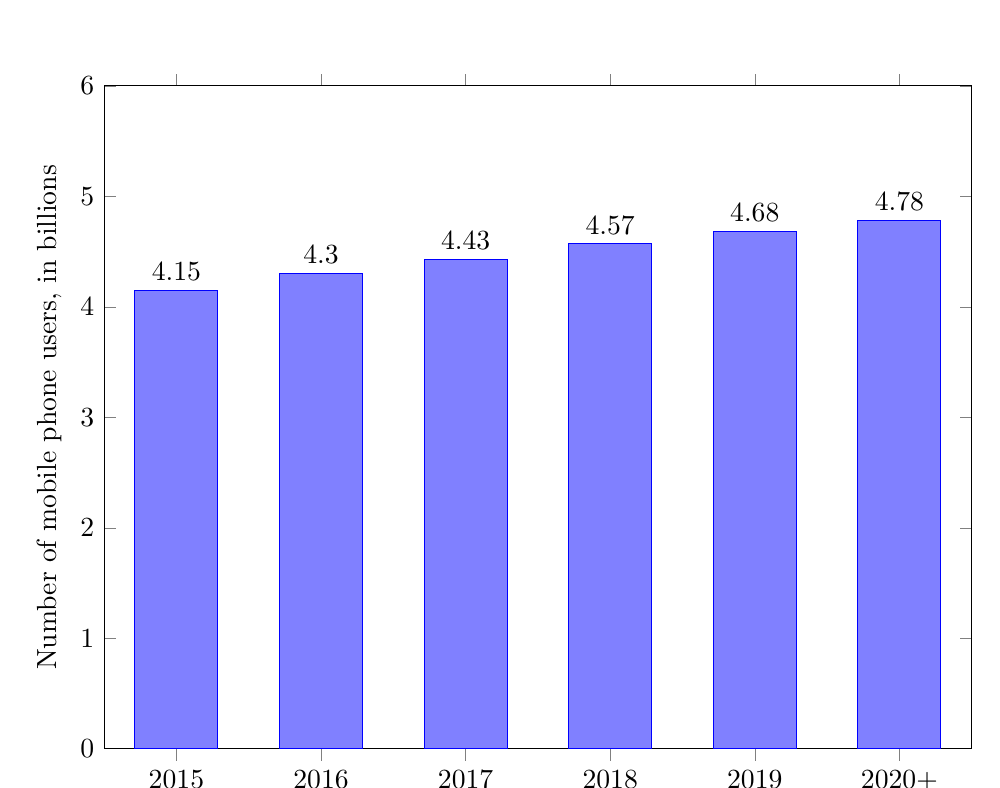
\begin{tikzpicture}
   \begin{axis}[
      ybar,
      bar width = 30,
      width=12.6cm,
      height=10cm,      
%       xlabel={year},
      ylabel={Number of mobile phone users, in billions},      
      symbolic x coords = {2015,2016,2017,2018,2019,2020+},
      ymin=0,
      ymax=6,
      nodes near coords,
      ]
      \addplot [draw=blue,fill=blue!50]
      coordinates {(2015,4.15) (2016,4.3) (2017,4.43) (2018,4.57) (2019,4.68) (2020+,4.78)};
   \end{axis}
\end{tikzpicture}
\caption*{Number of mobile phone users worldwide from 2015 to 2020 (in billions, \href{https://www.statista.com}{Statista.com})}
\end{figure}

Coupled with the \href{http://gs.statcounter.com/platform-market-share/desktop-mobile-tablet}{low entry threshold} a mobile device provides increased use of mobile devices in developing countries (more people have mobile phones \href{https://www.economist.com/graphic-detail/2017/11/08/in-much-of-sub-saharan-africa-mobile-phones-are-more-common-than-access-to-electricity}{than access to electricity} in Africa) it is becoming clear that mobile platforms will increase their market share in the future, to the point of becoming the absolute preferred method.

Taking the increasing popularity of mobile devices into account, it therefore makes sense for ODIN to focus its efforts on securing and anonymizing applications, data and services that primarily utilize the mobile platform.

ODIN will support applications that allow everything that could be done before, but without compromising your privacy or online security. It will also facilitate businesses and social models we have yet to dream about---similar to Sir Timothy John Berners-Lee being unable to anticipate game changing services like Netflix or Uber when he first \href{https://en.wikipedia.org/wiki/Tim_Berners-Lee}{invented the World Wide Web}.

Our blockchain will allow for the decentralization of applications and services avoiding the pitfalls of running applications through central organizations and server farms. Instead, data will be routed through any masternodes ran by the holders of the ODIN coin.

A range of toolkits will be created to lead you through a series of steps to build, test and launch your Dapps, including but not limited to:
\begin{itemize}
   \item Specific developer tools focusing on native languages
   \item UX designing and testing
   \item Prototyping and MVPs
   \item Business concept validation 
   \item Usability testing
   \item Marketing and promotion
   \item Agile implementation strategies
   \item OKR frameworks for aligned growth
   \item Acceptance testing/coding standards/documentation standards
   \item Mobile applications (on- or off-chain applications)
   \item How to support an online community
   \item Local exchange trading systems
   \item Community coins
   \item Growing a healthy community
\end{itemize}

A support infrastructure including but not limited to:
\begin{itemize}
   \item An active peer support developer community
   \item Financial assistance through community voted projects available through the community Vanir (\href{https://docs.google.com/document/d/15YAuXnc-3y06keG302AfK-6QCZ7PkonSIGuMRxncdcw/edit?disco=AAAACD6XbTI&ts=5b47a26b#heading=h.c0p3cw59hwku}{community portal}) supported via the OPL
   \item Education and partnership development
   \begin{itemize}
      \item Active links to universities and incubators
      \item Hosting hackathons
      \item Attending meetups to engage other projects and/or developers that may be interested in developing on the ODIN Blockchain
   \end{itemize}
\end{itemize}

We intend to bring the possibilities of the ODIN Blockchain to a greater audience, expanding far beyond the reach of crypto insiders. We will do this through focusing on the following three key areas: \textit{innovation}, \textit{intuitiveness}, and \textit{integrity}. 

\subsection{Innovation}
There are new and emerging opportunities for organizations and developers in all sectors to create and deliver compelling products, projects and services for their customers using the power of disruptive innovation brought by the use of blockchain technologies and by \textit{nurturing collaboration}.

The ODIN Alliance will advance ideas through research and peer-to-peer blockchain development with a rich and supportive range of partners, developers, business experts, and philanthropists. We aim to bridge the divide between Entrepreneurs (for profit and socially conscious) and innovative, agile, visionary developers.  

We empower all contributors to collaborate with us in shaping the future of ODIN.

\subsection{​Intuitive}
We understand very well the implications of using blockchain technology. As familiar as it is, it remains a new area of technology and thus people are generally reserved or even skeptical about its use case.

We intend to overturn this thinking by helping create applications that are user friendly, and that support and develop third-parties in creating out-of-the-box, `plug-and-play' software.

We aim to do this with our focus on usability to \textit{make blockchain usable}.

We will embody human-centered design across all our projects and frameworks in order to ensure intuitive ease of use and simplicity of experience. Supportive toolkits as expressed above are being built across all areas, from development through to design and community collaboration. These showcase ODIN's capabilities and help spur the growth of ODIN DApps and a library of smart contracts.

\subsubsection{Why is usability important?}
Usability is the measure of the quality of a user's experience when interacting with a product or system---whether a web site, software application, mobile technology, or any user-operated device.

There are many definitions for usability, but four elements can be broadly considered and which ODIN aims to address:
\begin{itemize}
   \item Intuitive and easy to learn
   \item Efficient to use
   \item Errors can be recovered from quickly
   \item Easy to remember
\end{itemize}
    
Whilst the end product Dapps will be out of our control, or more correctly in the control of the community, by focusing on usability we are more able to support creating projects, products and services where users will be satisfied, enjoy their interaction and achieve goals effectively and efficiently.  This will lead to more confidence and trust in what we are accomplishing.

Satisfied users are loyal users and increase the likelihood of recommending your product or service to others.

\subsubsection{The benefits of usability}
By focusing on usability, you will be benefited in many ways including:
\begin{itemize}
   \item Reduced development time and costs
   \item Reduced support costs
   \item Reduced user errors
   \item Reduced training time and costs
   \item Return on Investment
\end{itemize}

\subsubsection{​Integrity}

Whilst we have placed our focus on privacy and anonymization, the governance structure itself will be open and transparent. We will not ask people to blindly trust us to guide them, and consequently we will be open about our own goals and manners of achieving them. We always aim to `do the right things.'

This includes helping establish well respected open-source repositories and shaping governance and consensus decision-making models, so that we evolve into a truly decentralized community led organization.

Amongst others, we will:
\begin{itemize}
   \item Be transparent about funding and expenditures
   \item Create a community ethics board
   \item Welcome community suggestions
   \item Have the community to vote on proposals, effectively making OPL a catalyst for community initiatives and proponents to ensure all goes according to agreement, and making sure all funding is allocated to those projects the community chooses.
\end{itemize}
   
\subsection{​The ODIN Community}
As stated in the preface, the heart of ODIN is its community. ODIN will focus on four main communities:
\begin{itemize}
   \item The infrastructure community
   \item The Dapps community
   \item The end user community 
   \item The entrepreneurial community
\end{itemize}
All of whom require their own information, and have different motivations and needs.

ODIN already has an active and vibrant community which we aim to extend. We have a dedicated community manager aided by a group of very committed community moderators.

We constantly strive to help facilitate a positive, friendly, non-judgmental community who is willing and eager to support each other. 

Ultimately, ODIN Blockchain is directed by the community. As part of our commitment to \href{https://odinblockchain.org/#integrity}{Integrity}, we always want to be engaged, transparent and responsive to the needs of the community. We want you to shape our ideas and designs, and will constantly provide ways to gather feedback and to listen and understand what the ODIN Blockchain community wants.

\subsection{ODIN Community Portal}
To be a truly community led project, ODIN will provide a decentralized, recurring method to allocate funds for the development of valuable ideas and to help visualize the future direction of the ODIN ecosystem.

Community members that own the required amount of Odin for a masternode will be able to exercise their right to vote on what projects they wish to see pursued. A level of active education and engagement is required to make informed decisions for the future of the ODIN Ecosystem. 

Every masternode is entitled to one vote. Therefore, if you hold two masternodes you are given two votes. This allows for all levels of investment and genuine interest in the project’s success to have a bigger say, and reduces the odds of success for malicious actors to intentionally vote on terrible projects, obligating the Foundation to provide them with funds.

The funds for the pursuing of these projects will be taken out of stake rewards, and transferred to an openly visible address held by the Foundation.

Before each proposal cycle, any community member or aspiring developer may submit proposals that deliver value to the ODIN ecosystem. Listing a proposal will require submission of a 25 ODIN fee, which will be burned.

One proposal cycle will last for one month.

All these proposals will be publically viewable, and it is then left up to the community to debate and investigate these proposals for themselves. Masternode owners may then vote on these proposals.

At the end of each proposal cycle, voting is closed and the budget is finalized before being distributed. At this point the Foundation will submit a 25 ODIN fee which is burned, thus finalizing the budget for the cycle.

Masternodes automatically rank the proposals based on net yes versus no \%. Only the top three projects are then funded. The projects receive funds in a proportional way from the money raised during that cycle to, at most, the total value of the particular project and the remaining funds (if any) in the community wallet are rolled over to the following month.

For example, if four projects were submitted receiving the following votes
\begin{itemize}
   \item Project one -- 50\% of the vote
   \item Project two -- 20\% of the vote
   \item Project three -- 27\% of the vote
   \item Project four -- 3\% of the vote
\end{itemize}
Then the funds would be allocated as
\begin{itemize}
   \item Project one -- 51\% (50\% + 1\% of project four)
   \item Project two -- 21\% (20\% + 1\% of project four)
   \item Project three -- 28\% (27\% + 1\% of project four)
\end{itemize}

If however any \% vote caused a project to receive a larger fund than is needed, that money is rolled over to be available to the following month's allocation.

For example
\begin{itemize}
   \item Project one is to receive 51\% of the funds (which was, for example, 5000 ODIN) but that project only requested 4000 ODIN, 1000 ODIN would remain in the wallet until the following month.
   \item Periodically if the community wallet grows to an `excess' size we will engage with the community as to what you would like to do with these funds (options could include, roll over, burn etc)
\end{itemize}


\newpage
\section{ODIN Coin Distribution}
The Foundation will initially hold, and never exceed, 15\% of the total supply in a ``reserve wallet.'' This reserve wallet will ensure active development can be guaranteed even during times of low liquidity or possible market issues that may reduce cash flow.

The amount taken out of each stake reward for the governance pool will be 20\%.
\begin{itemize}
   \item 10\% of this is given directly back to the community in the form of a community treasury to support development of projects voted on by the masternode holders.
   \item 10\% is spent through the governance treasury to support operational costs of the Foundation (these costs will be made transparent through a Governance report at the end of each financial quarter).
   \item The Foundation's core reserve holdings will never exceed 15\% of the total supply, and will gradually decrease over time.
   \item The Foundation will never stake these core reserve holdings.
\end{itemize}

All the other coins in the total supply will be held strictly by the community.
\begin{center}
    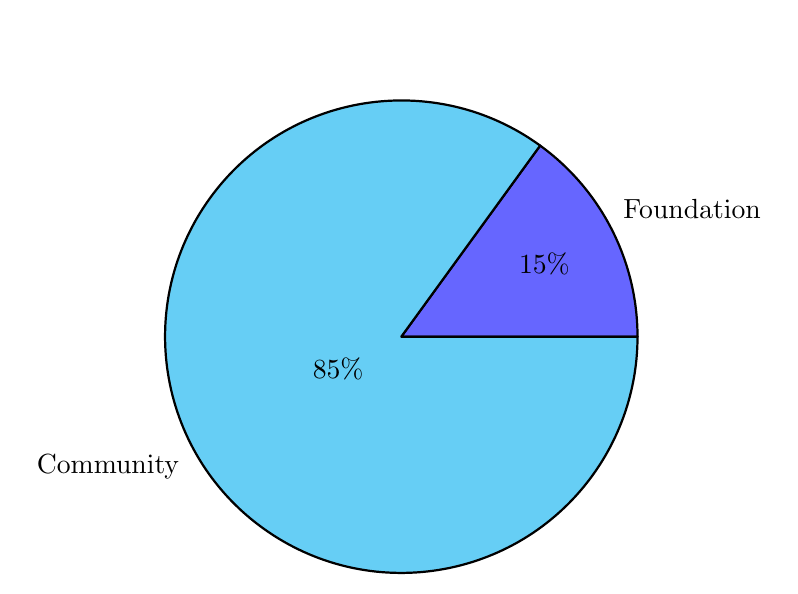
\begin{tikzpicture} 
       \pie{15/Foundation, 85/Community}
    \end{tikzpicture}
\end{center}


\newpage
\section{​Technical Overview}

\subsection{ODIN Coin}
The ODIN Coin (ODIN) is a PoS coin that uses the ODIN blockchain. ODIN is the native currency throughout the ODIN Ecosystem (OE) and is aimed, like the rest of the ecosystem, at mass adoption and real-world utilization. 
 
This will be promoted via the broad distribution of the ODIN Messenger (its first showcase app) and through the implementation of upcoming technologies and partnerships (see Roadmap).

\subsection{ODIN Mobile Messenger}
ODIN Mobile Messenger is an example decentralized application, (DApp), to demonstrate what can be built on top of the ODIN blockchain platform. It is a secure encrypted messenger which uses decentralized nodes, (at the time of writing, a stepping stone to upcoming ODIN service nodes), and allows signed messages on the blockchain. 
 
Once a connection is established, the system switches to peer to peer (P2P) communication between people and bots. All communications are encrypted, and users can choose to have their hash stored on the ODIN blockchain for a small fee. The ODIN  Mobile Messenger will have wallets built in, which allows for the sending and receipt of ODIN via both chat and wallets. 

\subsection{ODIN PoS Framework}
ODIN uses a Proof of Stake approach to secure the blockchain. This uses vastly less electricity then Proof of Work algorithms and is therefore more environmentally friendly and sustainable. It also facilitates greater decentralization since masternodes can be operated inexpensively. Transaction fees are also a fraction of bitcoin fees.

The ODN staking approach offers diverse options ranging from simple staking to more demanding masternoding schemes. A block reward (as described in the section \hyperlink{specifications}{ODIN Specifications}) will be split between masternodes and stakers where the exact ratios of the reward distribution will be adjusted over time.

\subsection{ODIN Staking Wallets}
Currently ODIN supports the ODIN-QT Windows, Linux, Mac and Android. This area is undergoing rapid development and updates are expected periodically.

Simplified staking framework is available through the wallets and it is encouraged to stake your coins both for the securing the network and to gain staking rewards.

Upcoming wallets:
\begin{itemize}
   \item Standalone Android wallet
   \item Standalone iOS wallet
   \item Raspberry Pi wallet
   \item Docker Wallet
   \item Paper wallet
   \item Online web wallet
   \item The ODIN messenger is set to feature a mobile ODIN wallet in 2018
   \item Hardware wallets (related to hardware partnerships):
   \begin{itemize}
      \item Trezor
      \item Keepkey
      \item Ledger Nano S.
   \end{itemize}
\end{itemize}

\subsection{​ODIN Masternodes}
We now have a well-calibrated masternode policy (see \hyperlink{specifications}{ODIN Specifications}) which was missing pre-fork.  

Our masternodes provide a decentralized network of servers separately held by individuals to provide the functional infrastructure of the ODIN blockchain.  As they provide additional services and security (supporting private transactions) they receive a greater reward than normal staking.   Given their large stake masternode owners have an incentive to maintain the security and integrity of the blockchain and guide its growth over time.

The more activity and resources that are required, the more fees are generated and the greater rewards are given. The algorithmic protocols balance exactly the ratio of rewards between stakers and masternodes. Using this approach a passive income stream is created.

In future releases, as we unveil additional ODIN features and products, masternodes will take on additional functional roles.

\subsubsection{What do ODIN masternodes do?}
Genuine masternodes holders have long term interests in mind. They are invested in the tech and the ecosystem and pay less attention to short term oscillations in value.  Therefore, masternodes themselves have a strong moderating effect on volatility in markets and the masternode community gradually grows into an informed and involved community. 

Currently they facilitate processing of transactions, they secure the network, they assist with unique features such as SwiftX and Obfuscation and they have a stabilizing influence over the coin volatility. 

Our masternodes also process zerocoin private transactions.

However, masternodes are more than just the IT infrastructure layer of an ecosystem; they provide the foundation upon which a strong and committed community can grow.

Intensive computing, storage and connectivity systems require a reliable infrastructure.  Masternodes provide these resources by creating a decentralized network of ``suppliers'' to the environment and are therefore providing a great tool against centralization whilst providing increased utility.

Our robust masternoding policy is setup to
\begin{itemize}
   \item Channel the ecosystem away from coin centralization 
   \item Offer a rational price that targets upper-mid range investors
   \item Prevent a potential over-exploitation of the PoS features by large coin holders
   \item Provide functional processes and offers a path towards platform fees
   \item Provide additional security, reliability and performance to the blockchain
   \item Ensure that a balance between sufficient liquidity and functional requirements.
\end{itemize}
If a masternode owner wishes to stop operating their masternode, they can unlock their coins and terminate the function at any time.

\subsubsection{How do you run an ODIN masternode?}
To run a masternode, one is required to lock sufficient amount of coin (\num{25000} ODIN per masternode) and follow the framework guidelines and operational criteria as per the upcoming published framework.

As masternodes are required to commit significant coin and uphold a functional criteria they receive a greater reward than normal staking.  This additional reward is to compensate for costs and effort. 

As running masternode requires significant holdings (\num{25000} ODIN per masternode) it is not `cheap' in terms of a monetary or a time commitment---hence there is incentive by this community to grow the impact of the project. However, due to a minimum amount of coins needed to run a masternode, it is also not feasible for large scale implementation. Therefore a large holder with hundreds of thousands or millions of coins would not be realistically able to run hundreds of servers and thereby over-ride decentralized consensus.  

\subsubsection{What is the reward for running an ODIN masternode?}
Masternodes receive block rewards as they provide functional roles on the various products that will make use of the masternode network and its offered functionalities. 
 
At any point, masternodes will have higher ROI compared to staking. This compensates them for providing the key functional role in the ODIN infrastructure and for their added commitment to promote more decentralized infrastructure.

The more activity and resources that are required, the more fees are generated and the greater rewards are given, algorithmic protocols balance exactly the ratio of rewards between stakers and masternodes so to ensure a healthy system that can grow and shrink as need be.

At the moment of writing 116.53 ODIN is rewarded for each block which is targeted to occur every 60 seconds. The return on investment for a masternode owner in the first year will change as masternodes are added and removed.

For clarity, the P2P and zODIN Transaction fees are burned.

\subsection{SwiftTX}
SwiftTX is a near-instantaneous and highly efficient mechanism for creating consensus and for locking-in transactions using a randomly selected masternode prior to being written into the blockchain.

This allows for great improvement in functional performance, allowing for near-real time transactions for non-critical operations (security of transaction's validity increases after being added into a block and greatly increases after ``maturing'' for a few blocks). This protocol will play an essential role in many operational elements to be developed and unveiled on the ODIN network.

After submission a subset of masternodes will validate the transaction and on reaching consensus they will lock this transaction for later addition to the blockchain.  Using this consensus mechanism multiple transaction can take place before block mine with the same inputs.  This approach greatly increases transaction speed compared with consensus mechanisms available in Bitcoin (for example)

\subsection{TOR \& IPV6 Masternodes}
Continuing with reinstating a privacy oriented environment, both nodes and masternodes can be run on IPV6 and onion address. Building a stable and smooth TOR network will require further development and mostly sufficient adoption by TOR masternodes, following which a significant layer of privacy, anonymity and security would be added.

Severing the link between the masternode hosting network through onionization as a complete TOR network would be most important to less secure domestic networks as well as improving overall anonymity of masternodes and opening many promising directions for future development of TOR oriented features.

\subsection{Sporks}
Sporking allows the network to quickly respond to security vulnerabilities and to implement new features in a smooth and low involvement from coin holders' and users' end.  Sporking is a multi-phased forking mechanism which in addition to minimising the risk of unintended network forks during rollouts, allows to respond to threats or issue patches without requiring nodes to run software updates.

Sporking is achieved by automatically changing a blockchain's behavior starting with a certain block. This specific block's number is not required to be known beforehand. Through this method, a blockchain's software can be automatically updated without any specific commands from the node operators. It is achieved merely through nodes receiving a message telling them when the software change comes into effect.

This method is extremely user friendly and goes hand in hand with our focus on \href{https://odinblockchain.org/#intuitive}{Intuitivity}. We wish to be as user friendly as possible in each aspect on our chain, from the blockchain's core features to the applications developed to run on top of the network.

\subsection{Zerocoin Protocol}
We all need privacy in certain elements of our lives.  Our belief is that this need for privacy also extends to elements of our life online.  In Bitcoin transactions information about the sender and receiver is publicly broadcast including the address where the bitcoin is coming from, the address it is going to and the amount sent. 

With proper scrutiny it is possible to reveal the identity of the owner over time. With cryptocurrencies that do not guarantee privacy, personal information can be analyzed, aggregated and ultimately sold without your knowledge or consent.

To guarantee privacy within transactions, ODIN uses a protocol called Zerocoin.  

Zerocoin completely breaks the transaction links between coins through the use of zero knowledge proofs. Simply speaking, zero knowledge proofs allow a party to prove a secret without revealing it to the other party.

Zerocoin mint allows you to burn coins and later redeem an equivalent amount of brand new coins (Zerocoin spend).  As these are brand new coins they have no prior transaction history.  In ODIN, Zerocoin verifies the transaction between the sender and receiver without revealing this link via the masternode infrastructure.  

Zerocoin minting is almost instantaneous and spending is a matter of seconds.
We have implanted a scaled level of security so the degrees to which you wish the coins to be mixed can be from five blocks before yours, to every coin in existence. For a small transaction ODIN can be minted in Zerocoin ODIN in a variety of standardized denominations.

Because of its additional computational energy required Minting Zerocoin ODIN (zODIN) is more expensive than a normal transaction.

Like other transaction fees, the zODIN fees are burned, reducing the total supply of ODIN. zODIN can be converted back later to ODIN, by sending them to their own wallet addresses, or to spend them at any other ODIN address, and spending zODIN has no transaction fee. Whilst they are held, zODIN are stored in the user's wallet like secure vouchers for ODIN that can be redeemed anonymously. If someone was concerned about being targeted by hackers, because they have a high balance in their account, using zODIN will mask their true balance, creating the ability to hold ``stealth'' value that cannot easily be traced back to the user's wallet.)

%%%%%%%%%%%%%%%%%%%%%%%%%%%%%%%%%%%%%%%%%%%%%%%%%%%%%%%%%%%%%%%%%%%%%%%%%%%%%%%%%%%%%%%%%%%%%%%%%%%%%%%%
% Tables are one of the weaknesses in LaTeX.  I actually did these in another program (LyX) and then
% copied and pasted the latex code here.  I didn't make it pretty... sorry!
\section{​ODIN Specifications}\hypertarget{specifications}{}
\begin{center}
\begin{adjustbox}{max width=\textwidth}
\begin{threeparttable}
\renewcommand{\arraystretch}{1.4}
\begin{tabular}{p{6.5cm} p{8cm}}
\hline
Item & Value \\
\hline
\hline
Trading Symbol                          & ODIN                  \\

Block Time                              & 60 Seconds            \\

Block Maturity                          & 50 confirmations      \\

Confirmation Time       & 6 Blocks ($\sim$6 Minutes) for P2P TXs, 51 Blocks ($\sim$51 Minutes) for Staking/Masternode Rewards\\

Block Size              & Maximum 2 MB \\

Premine Supply*          & \num{250000000} (estimated depending on total claim by the community) \tabularnewline

Current Supply**          & \num{250500000} \\

Block Reward            & 116 (decreases over time) \\

Masternode Reward Ratio & $48\% - xx$ ODIN$^\dag$\\

Staking Reward Ratio    & $32\% - xx$ ODIN$^\dag$ \\

Community Developer Fund Ratio & $10\% - xx$ ODIN$^\dag$ \\

Foundation Operating Costs     & $10\% - xx$ ODIN$^\dag$ \\

Transaction Fee         & $< 0.001^{\dag\dag}$ \\

Zerocoin Transaction fee & 0.01 zODIN$^{\dag\dag}$ \\

Masternode Requirement  & \num{25000} ODIN \\

PoW                     & Up to block 1500 \\

RPC Port                & 33221 \\

P2P Port                & 33222 \\

PoS Implementations     & Blackcoin v3.0 PoS \\

Supported Protocols     & IPV4, IPV6, TOR \\
\hline 
\end{tabular}
\begin{tablenotes}
   \item[*] Any unclaimed coins will be burned.
   \item[**] This will be reduced by a significant amount through a coin burn. This amount will be determined once we have a figure for the total ODIN that is being claimed by the community.
   \item[\dag] Amount will decrease overtime as Reward decreases, amount shown is current for current time of writing.
   \item[\dag\dag] P2P and zODIN transaction fees are burned
\end{tablenotes}
\end{threeparttable}
\end{adjustbox}
\end{center}
\renewcommand{\arraystretch}{1}

 
\subsection{ODIN Block generation/reward scheme}
\renewcommand{\arraystretch}{1.2}
\begin{center}
\begin{adjustbox}{max width=\textwidth}
\begin{threeparttable}
\begin{tabular}{|rrrrrrr|}
\hline 
Term & Reward & Block Reward & Estimated ROI$^\dag$ & From Block & To Block & Ending Supply$^{\dag\dag}$\tabularnewline
\hline 
\hline
Y1 Q1 & 15312500 & 116.53 & 70\% & 10000 & 141400 & 102812500\tabularnewline
\hline
Y1 Q2 & 15293359 & 116.39 & 60\% & 141401 & 272801 & 118105859\tabularnewline
\hline
Y1 Q3 & 14933010 & 113.65 & 51\% & 272802 & 404202 & 133038869\tabularnewline
\hline
Y1 Q4 & 14297937 & 108.81 & 43\% & 404203 & 535603 & 147336806\tabularnewline
\hline
Y2 Q1 & 13459378 & 102.43 & 37\% & 535604 & 667004 & 160796184\tabularnewline
\hline
Y2 Q2 & 12485571 & 95.02 & 31\% & 667005 & 798405 & 173281755\tabularnewline
\hline
Y2 Q3 & 11436798 & 87.04 & 26\% & 798406 & 929806 & 184718553\tabularnewline
\hline
Y2 Q4 & 10362894 & 78.87 & 22\% & 929807 & 1061207 & 195081447\tabularnewline
\hline
Y3 Q1 & 9302623 & 70.8 & 19\% & 1061208 & 1192608 & 204384070\tabularnewline
\hline
Y3 Q2 & 8284292 & 63.05 & 16\% & 1192609 & 1324009 & 212668362\tabularnewline
\hline
Y3 Q3 & 7327067 & 55.76 & 14\% & 1324010 & 1455410 & 219995430\tabularnewline
\hline
Y3 Q4 & 6442581 & 49.03 & 12\% & 1455411 & 1586811 & 226438011\tabularnewline
\hline
Y4 Q1 & 5660950 & 43.08 & 10\% & 1586812 & 1718212 & 232098961\tabularnewline
\hline
Y4 Q2 & 5802474 & 44.16 & 10\% & 1718213 & 1849613 & 237901435\tabularnewline
\hline
Y4 Q3 & 5947536 & 45.26 & 10\% & 1849614 & 1981014 & 243848971\tabularnewline
\hline
Y4 Q4 & 6096224 & 46.39 & 10\% & 1981015 & 2112415 & 249945195\tabularnewline
\hline
Y5 Q1 & 6248630 & 47.55 & 10\% & 2112416 & 2243816 & 256193825\tabularnewline
\hline
Y5 Q2 & 6404846 & 48.74 & 10\% & 2243817 & 2375217 & 262598671\tabularnewline
\hline
Y5 Q3 & 6564967 & 49.96 & 10\% & 2375218 & 2506618 & 269163637\tabularnewline
\hline
Y5 Q4 & 6729091 & 51.21 & 10\% & 2506619 & 2638019 & 275892728\tabularnewline
\hline
Y6 Q1 & 6897318 & 52.49 & 10\% & 2638020 & 2769420 & 282790047\tabularnewline
\hline
Y6 Q2 & 7069751 & 53.8 & 10\% & 2769421 & 2900821 & 289859798\tabularnewline
\hline
Y6 Q3 & 7246495 & 55.15 & 10\% & 2900822 & 3032222 & 297106293\tabularnewline
\hline
Y6 Q4 & 7427657 & 56.53 & 10\% & 3032223 & 3163623 & 304533950\tabularnewline
\hline
Y7 Q1 & 7613349 & 57.94 & 10\% & 3163624 & 3295024 & 312147299\tabularnewline
\hline
Y7 Q2 & 7803682 & 59.39 & 10\% & 3295025 & 3426425 & 319950981\tabularnewline
\hline
Y7 Q3 & 7998775 & 60.87 & 10\% & 3426426 & 3557826 & 327949756\tabularnewline
\hline
Y7 Q4 & 8198744 & 62.4 & 10\% & 3557827 & 3689227 & 336148500\tabularnewline
\hline
Y8 Q1 & 8403712 & 63.96 & 10\% & 3689228 & 3820628 & 344552212\tabularnewline
\hline
Y8 Q2 & 8613805 & 65.55 & 10\% & 3820629 & 3952029 & 353166018\tabularnewline
\hline
Y8 Q3 & 8829150 & 67.19 & 10\% & 3952030 & 4083430 & 361995168\tabularnewline
\hline
Y8 Q4 & 9049879 & 68.87 & 10\% & 4083431 & 4214831 & 371045047\tabularnewline
\hline
\end{tabular}
% }
\begin{tablenotes}
   \footnotesize 
   \item[\dag] Estimated ROI percentage is based on an estimation of number of masternodes running.
   \item[\dag\dag]Ending supply numbers are dependent on the amount of total ODIN claimed. 
   \normalsize
\end{tablenotes}
\end{threeparttable}
\end{adjustbox}
\end{center}
If, for instance, we take the amount held by the community as approximately 50M ODN, and 100\% of this is claimed, the community will receive a total of 125M ODIN. Making the initial total supply, in this instance 147M. 




\includepdf{tree.pdf}
% \newgeometry{margin=1.5cm}
%
\includegraphics[width=\textwidth]{tree}
% \restoregeometry
\end{document}
\grid
